\section{Appendix B - Part III}

\begin{figure}[H]
    \centering
    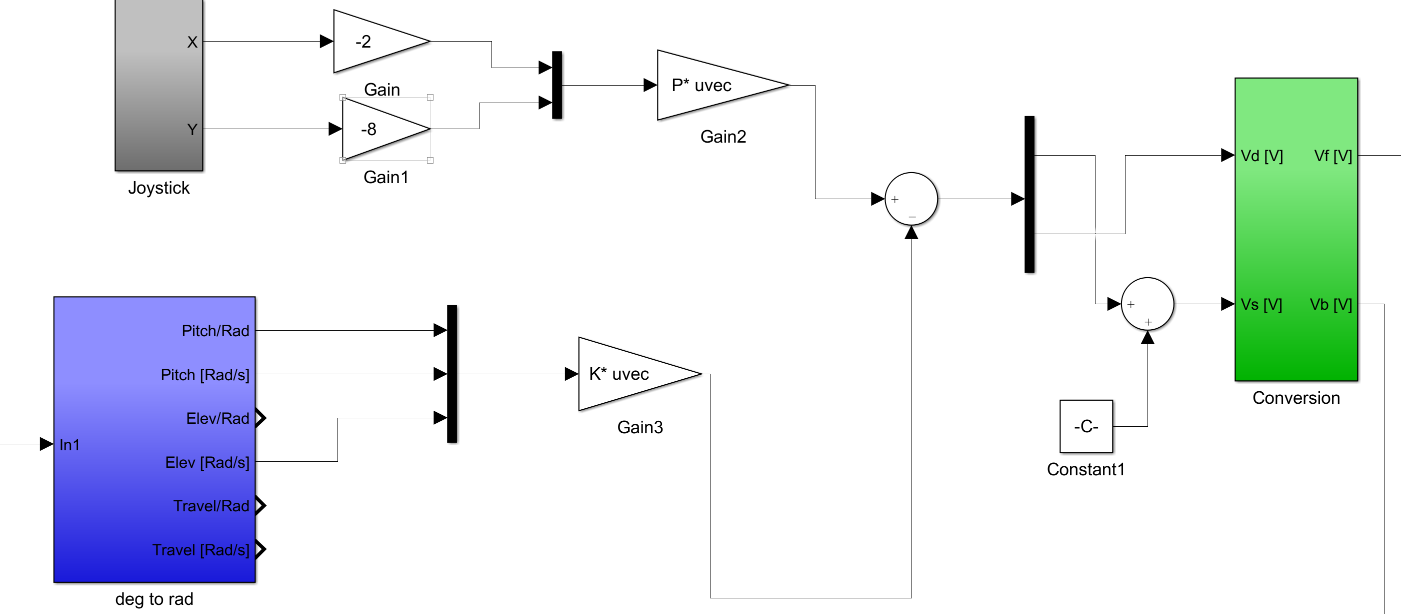
\includegraphics[width=1.2\textwidth]{figures/P3p2-LQR_preg}
    \caption{This is the LQR-controller, for part III - problem 2, implemented in Simulink}
    \label{fig:P3p2-LQR_preg}
\end{figure}

\begin{figure}[H]
    \centering
    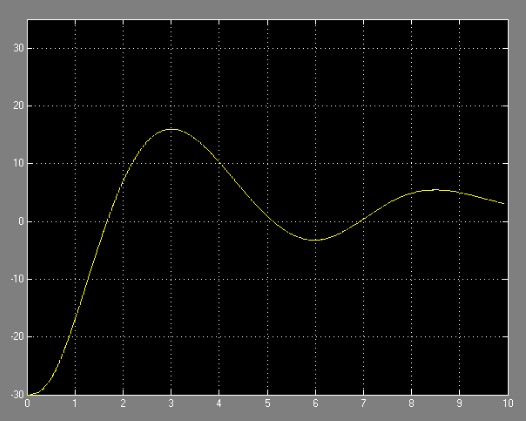
\includegraphics[width=0.8\textwidth]{figures/P3p2_elevation}
    \caption{The elevation of the LQR-controller, for part III - problem 2, with proportional effect}
    \label{fig:P3p2_elevation}
\end{figure}

\begin{figure}[H]
    \centering
    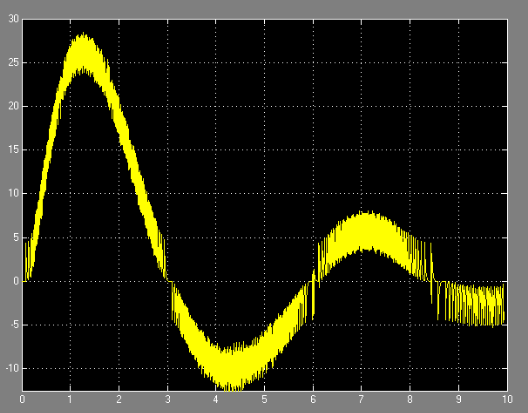
\includegraphics[width=0.8\textwidth]{figures/P3p2_elevationrate}
    \caption{The elevation rate of the LQR-controller, for part III - problem 2, with proportional effect}
    \label{fig:P3p3_elevationrate}
\end{figure}

\begin{figure}[H]
    \centering
    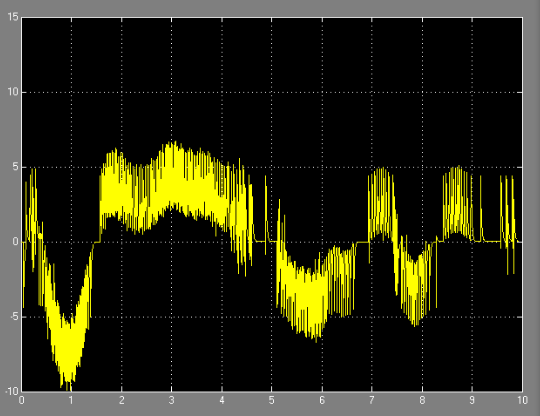
\includegraphics[width=0.8\textwidth]{figures/P3p2_pitchrate}
    \caption{The pitch rate of the LQR-controller, for part III - problem 2, with proportional effect}
    \label{fig:P3p2_pitchrate}
\end{figure}


\begin{figure}[H]
    \centering
    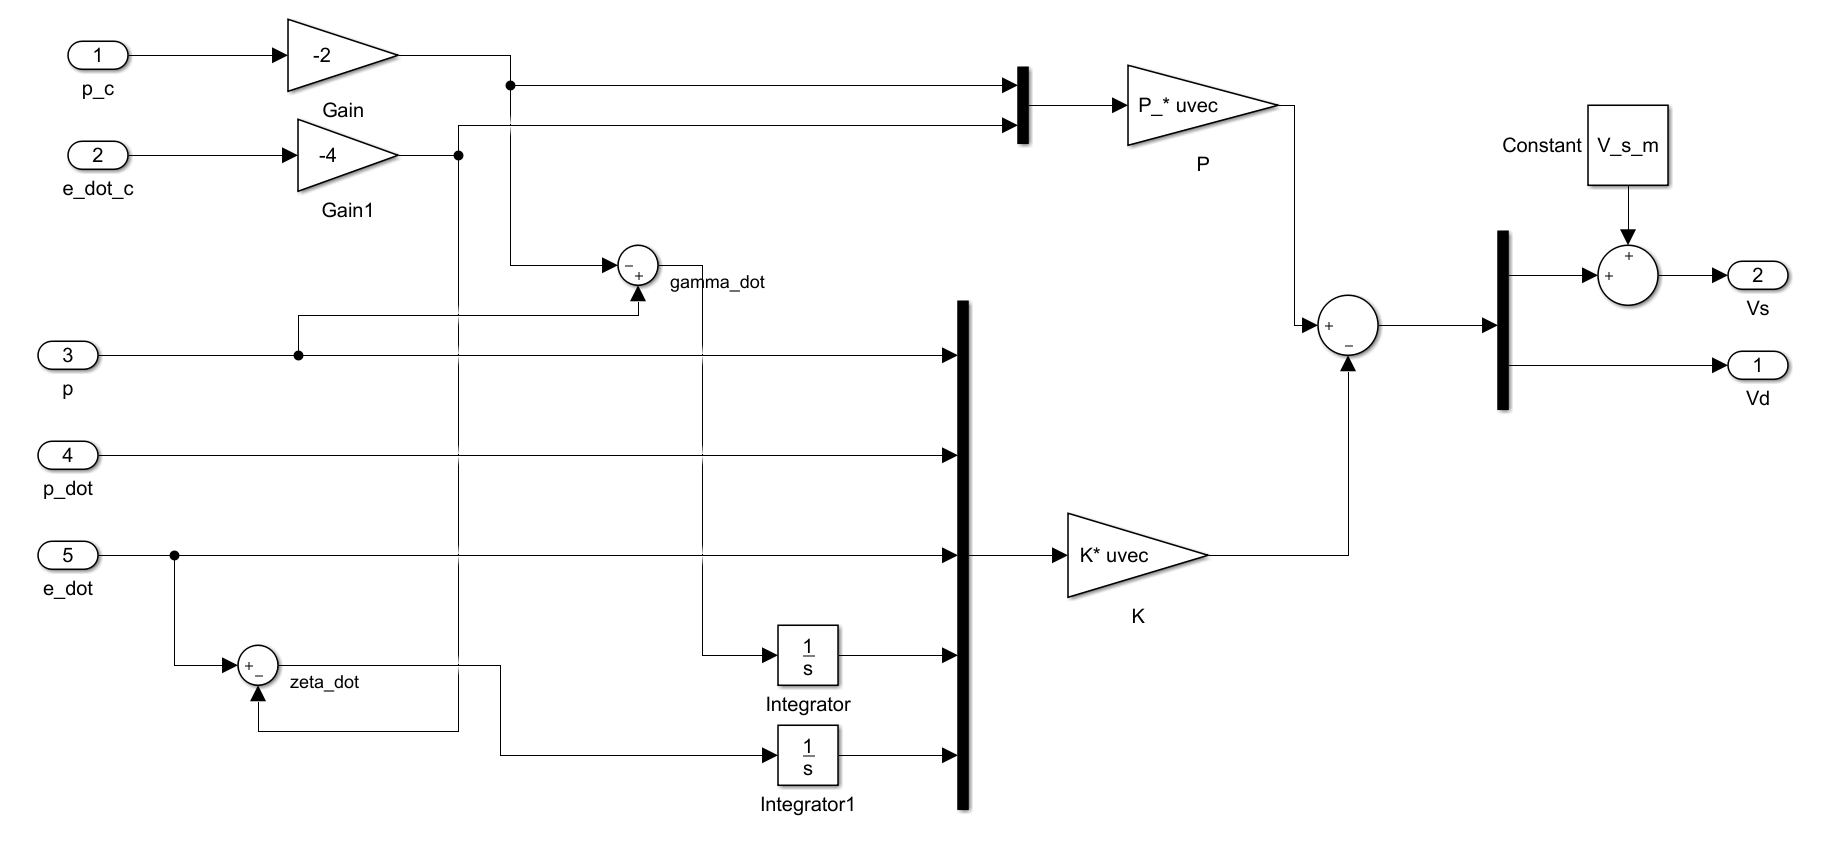
\includegraphics[width=1.2\textwidth]{figures/P3p3-LQR_PIreg}
    \caption{This is the LQR-controller, for part III - problem 3, implemented in Simulink}
    \label{fig:P3p3-LQR_PIreg}
\end{figure}

\begin{figure}[H]
    \centering
    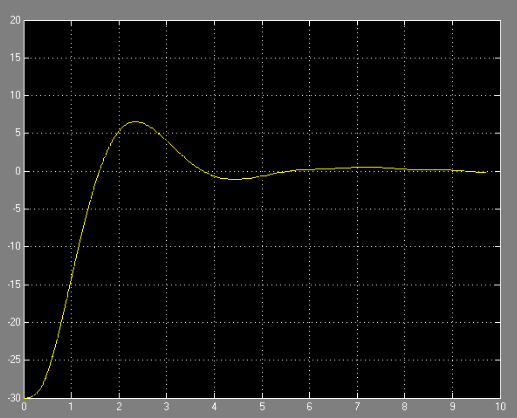
\includegraphics[width=0.8\textwidth]{figures/P3p3_elevation}
    \caption{The elevation of the LQR-controller, for part III - problem 3, with integral effect}
    \label{fig:P3p3_elevation}
\end{figure}

\begin{figure}[H]
    \centering
    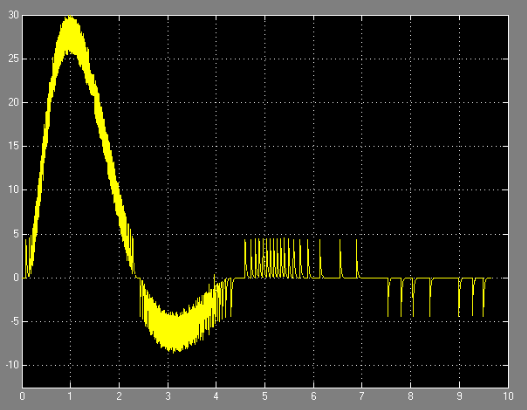
\includegraphics[width=0.8\textwidth]{figures/P3p3_elevationrate}
    \caption{The elevation rate of the LQR-controller, for part III - problem 3, with integral effect}
    \label{fig:P3p3_elevationrate}
\end{figure}

\begin{figure}[H]
    \centering
    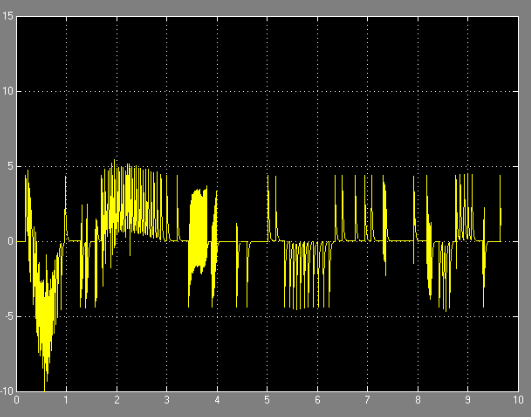
\includegraphics[width=0.8\textwidth]{figures/P3p3_pitchrate}
    \caption{The pitch rate of the LQR-controller, for part III - problem 3, with integral effect}
    \label{fig:P3p3_pitchrate}
\end{figure}
